% Options for packages loaded elsewhere
\PassOptionsToPackage{unicode}{hyperref}
\PassOptionsToPackage{hyphens}{url}
\PassOptionsToPackage{dvipsnames,svgnames,x11names}{xcolor}
%
\documentclass[
  letterpaper,
  DIV=11,
  numbers=noendperiod]{scrartcl}

\usepackage{amsmath,amssymb}
\usepackage{iftex}
\ifPDFTeX
  \usepackage[T1]{fontenc}
  \usepackage[utf8]{inputenc}
  \usepackage{textcomp} % provide euro and other symbols
\else % if luatex or xetex
  \usepackage{unicode-math}
  \defaultfontfeatures{Scale=MatchLowercase}
  \defaultfontfeatures[\rmfamily]{Ligatures=TeX,Scale=1}
\fi
\usepackage{lmodern}
\ifPDFTeX\else  
    % xetex/luatex font selection
\fi
% Use upquote if available, for straight quotes in verbatim environments
\IfFileExists{upquote.sty}{\usepackage{upquote}}{}
\IfFileExists{microtype.sty}{% use microtype if available
  \usepackage[]{microtype}
  \UseMicrotypeSet[protrusion]{basicmath} % disable protrusion for tt fonts
}{}
\makeatletter
\@ifundefined{KOMAClassName}{% if non-KOMA class
  \IfFileExists{parskip.sty}{%
    \usepackage{parskip}
  }{% else
    \setlength{\parindent}{0pt}
    \setlength{\parskip}{6pt plus 2pt minus 1pt}}
}{% if KOMA class
  \KOMAoptions{parskip=half}}
\makeatother
\usepackage{xcolor}
\setlength{\emergencystretch}{3em} % prevent overfull lines
\setcounter{secnumdepth}{-\maxdimen} % remove section numbering
% Make \paragraph and \subparagraph free-standing
\makeatletter
\ifx\paragraph\undefined\else
  \let\oldparagraph\paragraph
  \renewcommand{\paragraph}{
    \@ifstar
      \xxxParagraphStar
      \xxxParagraphNoStar
  }
  \newcommand{\xxxParagraphStar}[1]{\oldparagraph*{#1}\mbox{}}
  \newcommand{\xxxParagraphNoStar}[1]{\oldparagraph{#1}\mbox{}}
\fi
\ifx\subparagraph\undefined\else
  \let\oldsubparagraph\subparagraph
  \renewcommand{\subparagraph}{
    \@ifstar
      \xxxSubParagraphStar
      \xxxSubParagraphNoStar
  }
  \newcommand{\xxxSubParagraphStar}[1]{\oldsubparagraph*{#1}\mbox{}}
  \newcommand{\xxxSubParagraphNoStar}[1]{\oldsubparagraph{#1}\mbox{}}
\fi
\makeatother

\usepackage{color}
\usepackage{fancyvrb}
\newcommand{\VerbBar}{|}
\newcommand{\VERB}{\Verb[commandchars=\\\{\}]}
\DefineVerbatimEnvironment{Highlighting}{Verbatim}{commandchars=\\\{\}}
% Add ',fontsize=\small' for more characters per line
\usepackage{framed}
\definecolor{shadecolor}{RGB}{241,243,245}
\newenvironment{Shaded}{\begin{snugshade}}{\end{snugshade}}
\newcommand{\AlertTok}[1]{\textcolor[rgb]{0.68,0.00,0.00}{#1}}
\newcommand{\AnnotationTok}[1]{\textcolor[rgb]{0.37,0.37,0.37}{#1}}
\newcommand{\AttributeTok}[1]{\textcolor[rgb]{0.40,0.45,0.13}{#1}}
\newcommand{\BaseNTok}[1]{\textcolor[rgb]{0.68,0.00,0.00}{#1}}
\newcommand{\BuiltInTok}[1]{\textcolor[rgb]{0.00,0.23,0.31}{#1}}
\newcommand{\CharTok}[1]{\textcolor[rgb]{0.13,0.47,0.30}{#1}}
\newcommand{\CommentTok}[1]{\textcolor[rgb]{0.37,0.37,0.37}{#1}}
\newcommand{\CommentVarTok}[1]{\textcolor[rgb]{0.37,0.37,0.37}{\textit{#1}}}
\newcommand{\ConstantTok}[1]{\textcolor[rgb]{0.56,0.35,0.01}{#1}}
\newcommand{\ControlFlowTok}[1]{\textcolor[rgb]{0.00,0.23,0.31}{\textbf{#1}}}
\newcommand{\DataTypeTok}[1]{\textcolor[rgb]{0.68,0.00,0.00}{#1}}
\newcommand{\DecValTok}[1]{\textcolor[rgb]{0.68,0.00,0.00}{#1}}
\newcommand{\DocumentationTok}[1]{\textcolor[rgb]{0.37,0.37,0.37}{\textit{#1}}}
\newcommand{\ErrorTok}[1]{\textcolor[rgb]{0.68,0.00,0.00}{#1}}
\newcommand{\ExtensionTok}[1]{\textcolor[rgb]{0.00,0.23,0.31}{#1}}
\newcommand{\FloatTok}[1]{\textcolor[rgb]{0.68,0.00,0.00}{#1}}
\newcommand{\FunctionTok}[1]{\textcolor[rgb]{0.28,0.35,0.67}{#1}}
\newcommand{\ImportTok}[1]{\textcolor[rgb]{0.00,0.46,0.62}{#1}}
\newcommand{\InformationTok}[1]{\textcolor[rgb]{0.37,0.37,0.37}{#1}}
\newcommand{\KeywordTok}[1]{\textcolor[rgb]{0.00,0.23,0.31}{\textbf{#1}}}
\newcommand{\NormalTok}[1]{\textcolor[rgb]{0.00,0.23,0.31}{#1}}
\newcommand{\OperatorTok}[1]{\textcolor[rgb]{0.37,0.37,0.37}{#1}}
\newcommand{\OtherTok}[1]{\textcolor[rgb]{0.00,0.23,0.31}{#1}}
\newcommand{\PreprocessorTok}[1]{\textcolor[rgb]{0.68,0.00,0.00}{#1}}
\newcommand{\RegionMarkerTok}[1]{\textcolor[rgb]{0.00,0.23,0.31}{#1}}
\newcommand{\SpecialCharTok}[1]{\textcolor[rgb]{0.37,0.37,0.37}{#1}}
\newcommand{\SpecialStringTok}[1]{\textcolor[rgb]{0.13,0.47,0.30}{#1}}
\newcommand{\StringTok}[1]{\textcolor[rgb]{0.13,0.47,0.30}{#1}}
\newcommand{\VariableTok}[1]{\textcolor[rgb]{0.07,0.07,0.07}{#1}}
\newcommand{\VerbatimStringTok}[1]{\textcolor[rgb]{0.13,0.47,0.30}{#1}}
\newcommand{\WarningTok}[1]{\textcolor[rgb]{0.37,0.37,0.37}{\textit{#1}}}

\providecommand{\tightlist}{%
  \setlength{\itemsep}{0pt}\setlength{\parskip}{0pt}}\usepackage{longtable,booktabs,array}
\usepackage{calc} % for calculating minipage widths
% Correct order of tables after \paragraph or \subparagraph
\usepackage{etoolbox}
\makeatletter
\patchcmd\longtable{\par}{\if@noskipsec\mbox{}\fi\par}{}{}
\makeatother
% Allow footnotes in longtable head/foot
\IfFileExists{footnotehyper.sty}{\usepackage{footnotehyper}}{\usepackage{footnote}}
\makesavenoteenv{longtable}
\usepackage{graphicx}
\makeatletter
\def\maxwidth{\ifdim\Gin@nat@width>\linewidth\linewidth\else\Gin@nat@width\fi}
\def\maxheight{\ifdim\Gin@nat@height>\textheight\textheight\else\Gin@nat@height\fi}
\makeatother
% Scale images if necessary, so that they will not overflow the page
% margins by default, and it is still possible to overwrite the defaults
% using explicit options in \includegraphics[width, height, ...]{}
\setkeys{Gin}{width=\maxwidth,height=\maxheight,keepaspectratio}
% Set default figure placement to htbp
\makeatletter
\def\fps@figure{htbp}
\makeatother

\KOMAoption{captions}{tableheading}
\makeatletter
\@ifpackageloaded{caption}{}{\usepackage{caption}}
\AtBeginDocument{%
\ifdefined\contentsname
  \renewcommand*\contentsname{Table of contents}
\else
  \newcommand\contentsname{Table of contents}
\fi
\ifdefined\listfigurename
  \renewcommand*\listfigurename{List of Figures}
\else
  \newcommand\listfigurename{List of Figures}
\fi
\ifdefined\listtablename
  \renewcommand*\listtablename{List of Tables}
\else
  \newcommand\listtablename{List of Tables}
\fi
\ifdefined\figurename
  \renewcommand*\figurename{Figure}
\else
  \newcommand\figurename{Figure}
\fi
\ifdefined\tablename
  \renewcommand*\tablename{Table}
\else
  \newcommand\tablename{Table}
\fi
}
\@ifpackageloaded{float}{}{\usepackage{float}}
\floatstyle{ruled}
\@ifundefined{c@chapter}{\newfloat{codelisting}{h}{lop}}{\newfloat{codelisting}{h}{lop}[chapter]}
\floatname{codelisting}{Listing}
\newcommand*\listoflistings{\listof{codelisting}{List of Listings}}
\makeatother
\makeatletter
\makeatother
\makeatletter
\@ifpackageloaded{caption}{}{\usepackage{caption}}
\@ifpackageloaded{subcaption}{}{\usepackage{subcaption}}
\makeatother

\ifLuaTeX
  \usepackage{selnolig}  % disable illegal ligatures
\fi
\usepackage{bookmark}

\IfFileExists{xurl.sty}{\usepackage{xurl}}{} % add URL line breaks if available
\urlstyle{same} % disable monospaced font for URLs
\hypersetup{
  pdftitle={Solution: ggplot2},
  pdfauthor={Kevin Rue-Albrecht},
  colorlinks=true,
  linkcolor={blue},
  filecolor={Maroon},
  citecolor={Blue},
  urlcolor={Blue},
  pdfcreator={LaTeX via pandoc}}


\title{Solution: ggplot2}
\author{Kevin Rue-Albrecht}
\date{2025-02-10}

\begin{document}
\maketitle


\section{Exercise}\label{exercise}

Use \texttt{library(ggplot2)} to load the package.

\begin{Shaded}
\begin{Highlighting}[]
\FunctionTok{library}\NormalTok{(ggplot2)}
\end{Highlighting}
\end{Shaded}

\subsection{Specify the dataset.}\label{specify-the-dataset.}

What does \texttt{ggplot(diamonds)} do?

\begin{Shaded}
\begin{Highlighting}[]
\FunctionTok{ggplot}\NormalTok{(diamonds)}
\end{Highlighting}
\end{Shaded}

\includegraphics{5-ggplot2_kevin_files/figure-pdf/unnamed-chunk-3-1.pdf}

\begin{quote}
Answer: It creates a blank canvas for the plot. This is because we have
not defined which variables should be shown on each axis.
\end{quote}

\subsection{Add the aesthetics.}\label{add-the-aesthetics.}

What does \texttt{ggplot(diamonds,\ aes(x\ =\ carat,\ y\ =\ price))} do?

\begin{Shaded}
\begin{Highlighting}[]
\FunctionTok{ggplot}\NormalTok{(diamonds, }\FunctionTok{aes}\NormalTok{(}\AttributeTok{x =}\NormalTok{ carat, }\AttributeTok{y =}\NormalTok{ price))}
\end{Highlighting}
\end{Shaded}

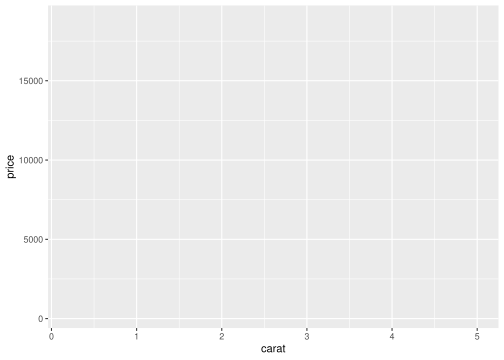
\includegraphics{5-ggplot2_kevin_files/figure-pdf/unnamed-chunk-4-1.pdf}

\begin{quote}
Answer: It adds axes in the x and y direction. Notably, the range of
each axis is set to fit the range of values observed for the associated
variable.
\end{quote}

\subsection{Add geometric objects}\label{add-geometric-objects}

\begin{itemize}
\tightlist
\item
  Add data points showing \texttt{carat} on the x-axis and
  \texttt{price} on the y-axis.
\end{itemize}

\begin{Shaded}
\begin{Highlighting}[]
\FunctionTok{ggplot}\NormalTok{(diamonds, }\FunctionTok{aes}\NormalTok{(}\AttributeTok{x =}\NormalTok{ carat, }\AttributeTok{y =}\NormalTok{ price)) }\SpecialCharTok{+}
  \FunctionTok{geom\_point}\NormalTok{()}
\end{Highlighting}
\end{Shaded}

\includegraphics{5-ggplot2_kevin_files/figure-pdf/unnamed-chunk-5-1.pdf}

\begin{itemize}
\tightlist
\item
  Color data points by \texttt{cut}. (Copy-paste and extend the code
  chunk above.)
\end{itemize}

\begin{Shaded}
\begin{Highlighting}[]
\FunctionTok{ggplot}\NormalTok{(diamonds, }\FunctionTok{aes}\NormalTok{(}\AttributeTok{x =}\NormalTok{ carat, }\AttributeTok{y =}\NormalTok{ price, }\AttributeTok{color =}\NormalTok{ cut)) }\SpecialCharTok{+}
  \FunctionTok{geom\_point}\NormalTok{()}
\end{Highlighting}
\end{Shaded}

\includegraphics{5-ggplot2_kevin_files/figure-pdf/unnamed-chunk-6-1.pdf}

\begin{itemize}
\tightlist
\item
  Add a smoothed mean trend line. (Copy-paste and extend the code chunk
  above.)
\end{itemize}

\begin{Shaded}
\begin{Highlighting}[]
\FunctionTok{ggplot}\NormalTok{(diamonds, }\FunctionTok{aes}\NormalTok{(}\AttributeTok{x =}\NormalTok{ carat, }\AttributeTok{y =}\NormalTok{ price, }\AttributeTok{color =}\NormalTok{ cut)) }\SpecialCharTok{+}
  \FunctionTok{geom\_point}\NormalTok{() }\SpecialCharTok{+}
  \FunctionTok{geom\_smooth}\NormalTok{()}
\end{Highlighting}
\end{Shaded}

\begin{verbatim}
`geom_smooth()` using method = 'gam' and formula = 'y ~ s(x, bs = "cs")'
\end{verbatim}

\includegraphics{5-ggplot2_kevin_files/figure-pdf/unnamed-chunk-7-1.pdf}

\begin{itemize}
\tightlist
\item
  Assign that last plot to an object called \texttt{obds\_diamonds}.
\end{itemize}

\begin{Shaded}
\begin{Highlighting}[]
\NormalTok{obds\_diamonds }\OtherTok{\textless{}{-}} \FunctionTok{ggplot}\NormalTok{(diamonds, }\FunctionTok{aes}\NormalTok{(}\AttributeTok{x =}\NormalTok{ carat, }\AttributeTok{y =}\NormalTok{ price, }\AttributeTok{color =}\NormalTok{ cut)) }\SpecialCharTok{+}
  \FunctionTok{geom\_point}\NormalTok{() }\SpecialCharTok{+}
  \FunctionTok{geom\_smooth}\NormalTok{()}
\end{Highlighting}
\end{Shaded}

\section{Exercise}\label{exercise-1}

Predict the difference between these two plots

\subsubsection{Plot 1}\label{plot-1}

\begin{Shaded}
\begin{Highlighting}[]
\FunctionTok{ggplot}\NormalTok{(diamonds, }\FunctionTok{aes}\NormalTok{(}\AttributeTok{x =}\NormalTok{ carat, }\AttributeTok{y =}\NormalTok{ price, }\AttributeTok{colour =}\NormalTok{ cut)) }\SpecialCharTok{+}
  \FunctionTok{geom\_point}\NormalTok{() }\SpecialCharTok{+}
  \FunctionTok{geom\_smooth}\NormalTok{()}
\end{Highlighting}
\end{Shaded}

\begin{verbatim}
`geom_smooth()` using method = 'gam' and formula = 'y ~ s(x, bs = "cs")'
\end{verbatim}

\includegraphics{5-ggplot2_kevin_files/figure-pdf/unnamed-chunk-9-1.pdf}

\subsubsection{Plot 2}\label{plot-2}

\begin{Shaded}
\begin{Highlighting}[]
\FunctionTok{ggplot}\NormalTok{(diamonds, }\FunctionTok{aes}\NormalTok{(}\AttributeTok{x =}\NormalTok{ carat, }\AttributeTok{y =}\NormalTok{ price)) }\SpecialCharTok{+}
  \FunctionTok{geom\_point}\NormalTok{(}\FunctionTok{aes}\NormalTok{(}\AttributeTok{colour =}\NormalTok{ cut)) }\SpecialCharTok{+}
  \FunctionTok{geom\_smooth}\NormalTok{()}
\end{Highlighting}
\end{Shaded}

\begin{verbatim}
`geom_smooth()` using method = 'gam' and formula = 'y ~ s(x, bs = "cs")'
\end{verbatim}

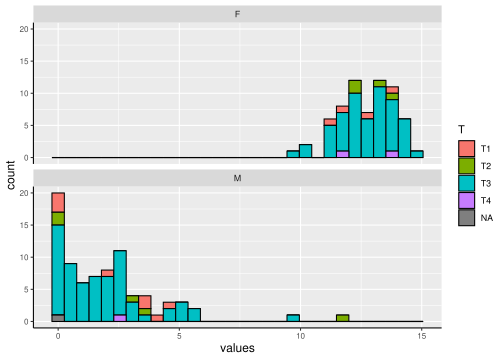
\includegraphics{5-ggplot2_kevin_files/figure-pdf/unnamed-chunk-10-1.pdf}

\begin{quote}
Answer: When the colour is specified as an aesthetic in the
\texttt{ggplot()} call, the aesthetic is applied to all layers in the
plot, resulting in coloured lines matching the coloured data points.
When the colour is specified as an aesthetic specifically in the
\texttt{geom\_point()} call, the aesthetic is only known to that layer,
and only the data points are coloured. As a result, only a single line
is computed and displayed, in the default colour (blue).
\end{quote}

\section{Exercise}\label{exercise-2}

\subsection{Trend lines}\label{trend-lines}

Using the \texttt{ChickWeight} data set:

\begin{itemize}
\tightlist
\item
  Create a scatter plot of weight (y-axis) over time (x-axis).
\end{itemize}

\begin{Shaded}
\begin{Highlighting}[]
\FunctionTok{ggplot}\NormalTok{(ChickWeight, }\FunctionTok{aes}\NormalTok{(Time, weight)) }\SpecialCharTok{+}
  \FunctionTok{geom\_point}\NormalTok{()}
\end{Highlighting}
\end{Shaded}

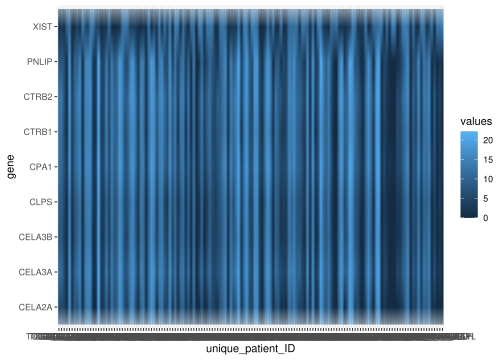
\includegraphics{5-ggplot2_kevin_files/figure-pdf/unnamed-chunk-11-1.pdf}

\begin{itemize}
\tightlist
\item
  Color by diet. (Copy-paste and extend the code chunk above.)
\end{itemize}

\begin{Shaded}
\begin{Highlighting}[]
\FunctionTok{ggplot}\NormalTok{(ChickWeight) }\SpecialCharTok{+}
  \FunctionTok{geom\_point}\NormalTok{(}\FunctionTok{aes}\NormalTok{(Time, weight, }\AttributeTok{color =}\NormalTok{ Diet))}
\end{Highlighting}
\end{Shaded}

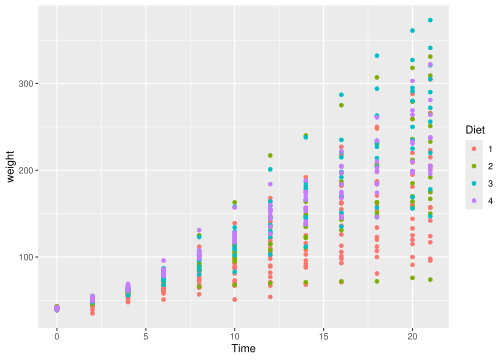
\includegraphics{5-ggplot2_kevin_files/figure-pdf/unnamed-chunk-12-1.pdf}

\begin{itemize}
\tightlist
\item
  Add a linear mean trend line for each diet. (Copy-paste and extend the
  code chunk above.)
\end{itemize}

\begin{Shaded}
\begin{Highlighting}[]
\FunctionTok{ggplot}\NormalTok{(ChickWeight, }\FunctionTok{aes}\NormalTok{(Time, weight, }\AttributeTok{color =}\NormalTok{ Diet)) }\SpecialCharTok{+}
  \FunctionTok{geom\_point}\NormalTok{() }\SpecialCharTok{+}
  \FunctionTok{geom\_smooth}\NormalTok{(}\AttributeTok{method =} \StringTok{"lm"}\NormalTok{, }\AttributeTok{formula =}\NormalTok{ y }\SpecialCharTok{\textasciitilde{}}\NormalTok{ x)}
\end{Highlighting}
\end{Shaded}

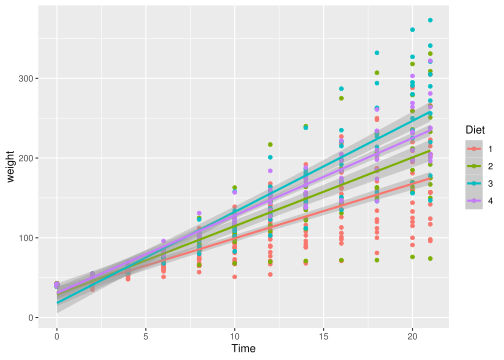
\includegraphics{5-ggplot2_kevin_files/figure-pdf/unnamed-chunk-13-1.pdf}

At this point you should be able to visually identify the diet that
leads to the highest mean increase in weight.

\begin{quote}
Answer: Diet 3
\end{quote}

\begin{itemize}
\tightlist
\item
  Facet a ribbon of sub-plots, one per diet. (Copy-paste and extend the
  code chunk above.)
\end{itemize}

\begin{Shaded}
\begin{Highlighting}[]
\FunctionTok{ggplot}\NormalTok{(ChickWeight, }\FunctionTok{aes}\NormalTok{(Time, weight, }\AttributeTok{color =}\NormalTok{ Diet)) }\SpecialCharTok{+}
  \FunctionTok{geom\_point}\NormalTok{() }\SpecialCharTok{+}
  \FunctionTok{geom\_smooth}\NormalTok{(}\AttributeTok{method =} \StringTok{"lm"}\NormalTok{, }\AttributeTok{formula =}\NormalTok{ y }\SpecialCharTok{\textasciitilde{}}\NormalTok{ x) }\SpecialCharTok{+}
  \FunctionTok{facet\_wrap}\NormalTok{(}\SpecialCharTok{\textasciitilde{}}\NormalTok{Diet)}
\end{Highlighting}
\end{Shaded}

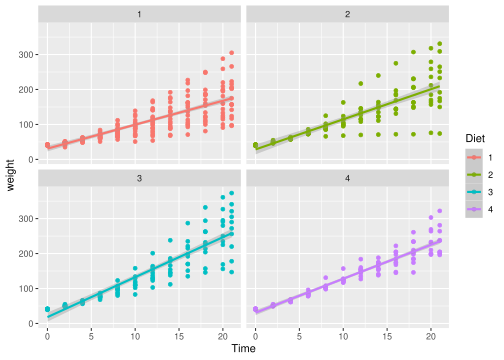
\includegraphics{5-ggplot2_kevin_files/figure-pdf/unnamed-chunk-14-1.pdf}

\begin{itemize}
\tightlist
\item
  Assign that last plot to an object called \texttt{obds\_chickweight}.
\end{itemize}

\begin{Shaded}
\begin{Highlighting}[]
\NormalTok{obds\_chickweight }\OtherTok{\textless{}{-}} \FunctionTok{ggplot}\NormalTok{(ChickWeight, }\FunctionTok{aes}\NormalTok{(Time, weight, }\AttributeTok{color =}\NormalTok{ Diet)) }\SpecialCharTok{+}
  \FunctionTok{geom\_point}\NormalTok{() }\SpecialCharTok{+}
  \FunctionTok{geom\_smooth}\NormalTok{(}\AttributeTok{method =} \StringTok{"lm"}\NormalTok{, }\AttributeTok{formula =}\NormalTok{ y }\SpecialCharTok{\textasciitilde{}}\NormalTok{ x) }\SpecialCharTok{+}
  \FunctionTok{facet\_wrap}\NormalTok{(}\SpecialCharTok{\textasciitilde{}}\NormalTok{Diet)}
\end{Highlighting}
\end{Shaded}

\section{Exercise}\label{exercise-3}

\subsection{Bar plot}\label{bar-plot}

\begin{itemize}
\tightlist
\item
  Load the \texttt{ggplot2::msleep} data set.
\end{itemize}

\begin{Shaded}
\begin{Highlighting}[]
\FunctionTok{data}\NormalTok{(msleep)}
\end{Highlighting}
\end{Shaded}

\begin{itemize}
\tightlist
\item
  Draw a bar plot of number of observations (i.e., rows) for each
  taxonomic order (i.e, one plot and one bar per taxonomic order).
\end{itemize}

\begin{Shaded}
\begin{Highlighting}[]
\FunctionTok{ggplot}\NormalTok{(msleep, }\FunctionTok{aes}\NormalTok{(order)) }\SpecialCharTok{+}
  \FunctionTok{geom\_bar}\NormalTok{()}
\end{Highlighting}
\end{Shaded}

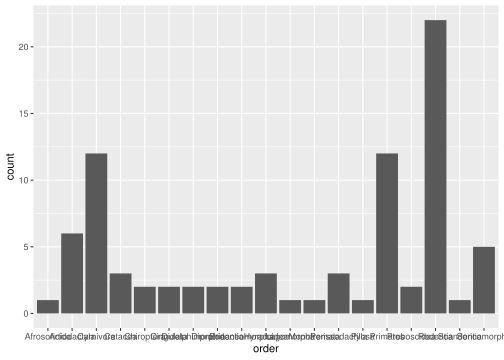
\includegraphics{5-ggplot2_kevin_files/figure-pdf/unnamed-chunk-17-1.pdf}

\begin{itemize}
\tightlist
\item
  Change the angle and font size of the text for the x-axis ticks (not
  the axis titles). Justify the text of those x-axis ticks as
  right-aligned. (Copy-paste and extend the code chunk above.)
\end{itemize}

\begin{Shaded}
\begin{Highlighting}[]
\FunctionTok{ggplot}\NormalTok{(msleep, }\FunctionTok{aes}\NormalTok{(order)) }\SpecialCharTok{+}
  \FunctionTok{geom\_bar}\NormalTok{() }\SpecialCharTok{+}
  \FunctionTok{theme}\NormalTok{(}
    \AttributeTok{axis.text.x =} \FunctionTok{element\_text}\NormalTok{(}\AttributeTok{size =} \FunctionTok{rel}\NormalTok{(}\FloatTok{1.5}\NormalTok{), }\AttributeTok{angle =} \DecValTok{60}\NormalTok{, }\AttributeTok{hjust =} \DecValTok{1}\NormalTok{, }\AttributeTok{vjust =} \DecValTok{1}\NormalTok{)}
\NormalTok{    )}
\end{Highlighting}
\end{Shaded}

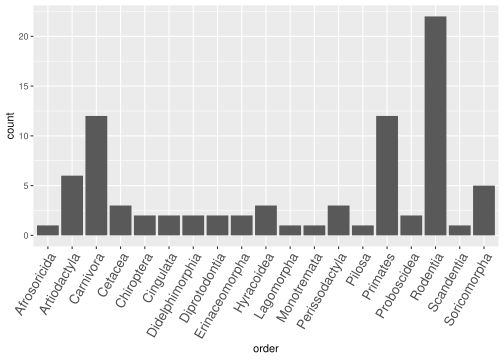
\includegraphics{5-ggplot2_kevin_files/figure-pdf/unnamed-chunk-18-1.pdf}

\begin{itemize}
\tightlist
\item
  Change the value and font size of the title for both x and y axes.
  (Copy-paste and extend the code chunk above.)
\end{itemize}

\begin{Shaded}
\begin{Highlighting}[]
\FunctionTok{ggplot}\NormalTok{(msleep, }\FunctionTok{aes}\NormalTok{(order)) }\SpecialCharTok{+}
  \FunctionTok{geom\_bar}\NormalTok{() }\SpecialCharTok{+}
  \FunctionTok{labs}\NormalTok{(}\AttributeTok{x =} \StringTok{"Taxonomic order"}\NormalTok{, }\AttributeTok{y =} \StringTok{"Observations"}\NormalTok{) }\SpecialCharTok{+}
  \FunctionTok{theme}\NormalTok{(}
    \AttributeTok{axis.text.x =} \FunctionTok{element\_text}\NormalTok{(}\AttributeTok{size =} \FunctionTok{rel}\NormalTok{(}\FloatTok{1.5}\NormalTok{), }\AttributeTok{angle =} \DecValTok{60}\NormalTok{, }\AttributeTok{hjust =} \DecValTok{1}\NormalTok{, }\AttributeTok{vjust =} \DecValTok{1}\NormalTok{),}
    \AttributeTok{axis.title =} \FunctionTok{element\_text}\NormalTok{(}\AttributeTok{size =} \FunctionTok{rel}\NormalTok{(}\DecValTok{2}\NormalTok{))}
\NormalTok{    )}
\end{Highlighting}
\end{Shaded}

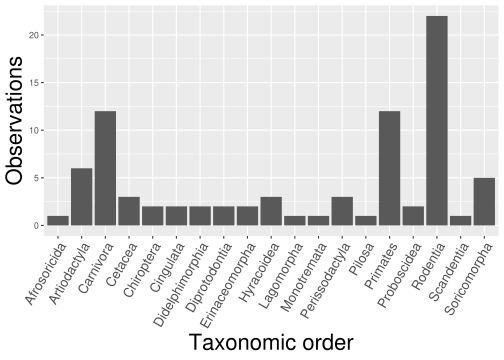
\includegraphics{5-ggplot2_kevin_files/figure-pdf/unnamed-chunk-19-1.pdf}

\begin{itemize}
\tightlist
\item
  Fill each bar with colors, proportionally to the count of each genus.
  (Copy-paste and extend the code chunk above.)
\end{itemize}

\begin{Shaded}
\begin{Highlighting}[]
\FunctionTok{ggplot}\NormalTok{(msleep, }\FunctionTok{aes}\NormalTok{(order)) }\SpecialCharTok{+}
  \FunctionTok{geom\_bar}\NormalTok{(}\FunctionTok{aes}\NormalTok{(}\AttributeTok{fill =}\NormalTok{ genus)) }\SpecialCharTok{+}
  \FunctionTok{labs}\NormalTok{(}\AttributeTok{x =} \StringTok{"Taxonomic order"}\NormalTok{, }\AttributeTok{y =} \StringTok{"Observations"}\NormalTok{) }\SpecialCharTok{+}
  \FunctionTok{theme}\NormalTok{(}
    \AttributeTok{axis.text.x =} \FunctionTok{element\_text}\NormalTok{(}\AttributeTok{size =} \FunctionTok{rel}\NormalTok{(}\FloatTok{1.5}\NormalTok{), }\AttributeTok{angle =} \DecValTok{60}\NormalTok{, }\AttributeTok{hjust =} \DecValTok{1}\NormalTok{, }\AttributeTok{vjust =} \DecValTok{1}\NormalTok{),}
    \AttributeTok{axis.title =} \FunctionTok{element\_text}\NormalTok{(}\AttributeTok{size =} \FunctionTok{rel}\NormalTok{(}\DecValTok{2}\NormalTok{))}
\NormalTok{    ) }
\end{Highlighting}
\end{Shaded}

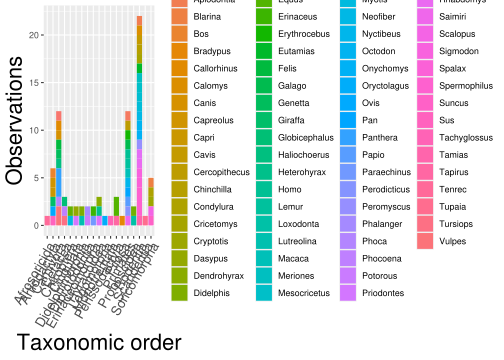
\includegraphics{5-ggplot2_kevin_files/figure-pdf/unnamed-chunk-20-1.pdf}

From this point onwards, you may need to iteratively resize the text of
the ticks and axes for readability.

\begin{itemize}
\tightlist
\item
  Reduce the legend key size. (Recommendation: use
  \texttt{unit(2,\ "mm")}). (Copy-paste and extend the code chunk
  above.)
\end{itemize}

\begin{Shaded}
\begin{Highlighting}[]
\FunctionTok{ggplot}\NormalTok{(msleep, }\FunctionTok{aes}\NormalTok{(order)) }\SpecialCharTok{+}
  \FunctionTok{geom\_bar}\NormalTok{(}\FunctionTok{aes}\NormalTok{(}\AttributeTok{fill =}\NormalTok{ genus)) }\SpecialCharTok{+}
  \FunctionTok{labs}\NormalTok{(}\AttributeTok{x =} \StringTok{"Taxonomic order"}\NormalTok{, }\AttributeTok{y =} \StringTok{"Observations"}\NormalTok{) }\SpecialCharTok{+}
  \FunctionTok{theme}\NormalTok{(}
    \AttributeTok{axis.text.x =} \FunctionTok{element\_text}\NormalTok{(}\AttributeTok{size =} \FunctionTok{rel}\NormalTok{(}\FloatTok{1.5}\NormalTok{), }\AttributeTok{angle =} \DecValTok{60}\NormalTok{, }\AttributeTok{hjust =} \DecValTok{1}\NormalTok{, }\AttributeTok{vjust =} \DecValTok{1}\NormalTok{),}
    \AttributeTok{axis.title =} \FunctionTok{element\_text}\NormalTok{(}\AttributeTok{size =} \FunctionTok{rel}\NormalTok{(}\DecValTok{2}\NormalTok{)),}
    \AttributeTok{legend.key.size =} \FunctionTok{unit}\NormalTok{(}\DecValTok{2}\NormalTok{, }\StringTok{"mm"}\NormalTok{)}
\NormalTok{    )}
\end{Highlighting}
\end{Shaded}

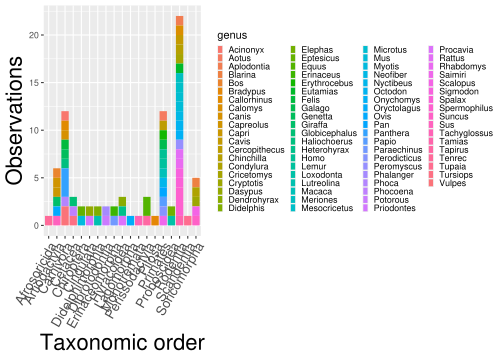
\includegraphics{5-ggplot2_kevin_files/figure-pdf/unnamed-chunk-21-1.pdf}

\begin{itemize}
\tightlist
\item
  Force the legend to be display in 3 columns. (Recommendation: use
  \texttt{guide\_legend(...)}). (Copy-paste and extend the code chunk
  above.)
\end{itemize}

\begin{Shaded}
\begin{Highlighting}[]
\FunctionTok{ggplot}\NormalTok{(msleep, }\FunctionTok{aes}\NormalTok{(order)) }\SpecialCharTok{+}
  \FunctionTok{geom\_bar}\NormalTok{(}\FunctionTok{aes}\NormalTok{(}\AttributeTok{fill =}\NormalTok{ genus)) }\SpecialCharTok{+}
  \FunctionTok{labs}\NormalTok{(}\AttributeTok{x =} \StringTok{"Taxonomic order"}\NormalTok{, }\AttributeTok{y =} \StringTok{"Observations"}\NormalTok{) }\SpecialCharTok{+}
  \FunctionTok{theme}\NormalTok{(}
    \AttributeTok{axis.text.x =} \FunctionTok{element\_text}\NormalTok{(}\AttributeTok{size =} \FunctionTok{rel}\NormalTok{(}\FloatTok{1.2}\NormalTok{), }\AttributeTok{angle =} \DecValTok{60}\NormalTok{, }\AttributeTok{hjust =} \DecValTok{1}\NormalTok{, }\AttributeTok{vjust =} \DecValTok{1}\NormalTok{),}
    \AttributeTok{axis.text.y =} \FunctionTok{element\_text}\NormalTok{(}\AttributeTok{size =} \FunctionTok{rel}\NormalTok{(}\FloatTok{1.2}\NormalTok{)),}
    \AttributeTok{axis.title =} \FunctionTok{element\_text}\NormalTok{(}\AttributeTok{size =} \FunctionTok{rel}\NormalTok{(}\FloatTok{1.5}\NormalTok{)),}
    \AttributeTok{legend.key.size =} \FunctionTok{unit}\NormalTok{(}\DecValTok{2}\NormalTok{, }\StringTok{"mm"}\NormalTok{)}
\NormalTok{    ) }\SpecialCharTok{+}
  \FunctionTok{guides}\NormalTok{(}\AttributeTok{fill =} \FunctionTok{guide\_legend}\NormalTok{(}\AttributeTok{ncol =} \DecValTok{3}\NormalTok{))}
\end{Highlighting}
\end{Shaded}

\includegraphics{5-ggplot2_kevin_files/figure-pdf/unnamed-chunk-22-1.pdf}

\begin{itemize}
\tightlist
\item
  Add a contour of thin black lines to the bars.
\end{itemize}

\begin{Shaded}
\begin{Highlighting}[]
\FunctionTok{ggplot}\NormalTok{(msleep, }\FunctionTok{aes}\NormalTok{(order)) }\SpecialCharTok{+}
  \FunctionTok{geom\_bar}\NormalTok{(}\FunctionTok{aes}\NormalTok{(}\AttributeTok{fill =}\NormalTok{ genus), }\AttributeTok{color =} \StringTok{"black"}\NormalTok{, }\AttributeTok{size =} \FloatTok{0.2}\NormalTok{) }\SpecialCharTok{+}
  \FunctionTok{labs}\NormalTok{(}\AttributeTok{x =} \StringTok{"Taxonomic order"}\NormalTok{, }\AttributeTok{y =} \StringTok{"Observations"}\NormalTok{) }\SpecialCharTok{+}
  \FunctionTok{theme}\NormalTok{(}
    \AttributeTok{axis.text.x =} \FunctionTok{element\_text}\NormalTok{(}\AttributeTok{size =} \FunctionTok{rel}\NormalTok{(}\FloatTok{1.2}\NormalTok{), }\AttributeTok{angle =} \DecValTok{60}\NormalTok{, }\AttributeTok{hjust =} \DecValTok{1}\NormalTok{, }\AttributeTok{vjust =} \DecValTok{1}\NormalTok{),}
    \AttributeTok{axis.text.y =} \FunctionTok{element\_text}\NormalTok{(}\AttributeTok{size =} \FunctionTok{rel}\NormalTok{(}\FloatTok{1.2}\NormalTok{)),}
    \AttributeTok{axis.title =} \FunctionTok{element\_text}\NormalTok{(}\AttributeTok{size =} \FunctionTok{rel}\NormalTok{(}\FloatTok{1.5}\NormalTok{)),}
    \AttributeTok{legend.key.size =} \FunctionTok{unit}\NormalTok{(}\DecValTok{2}\NormalTok{, }\StringTok{"mm"}\NormalTok{)}
\NormalTok{    ) }\SpecialCharTok{+}
  \FunctionTok{guides}\NormalTok{(}\AttributeTok{fill =} \FunctionTok{guide\_legend}\NormalTok{(}\AttributeTok{ncol =} \DecValTok{3}\NormalTok{))}
\end{Highlighting}
\end{Shaded}

\begin{verbatim}
Warning: Using `size` aesthetic for lines was deprecated in ggplot2 3.4.0.
i Please use `linewidth` instead.
\end{verbatim}

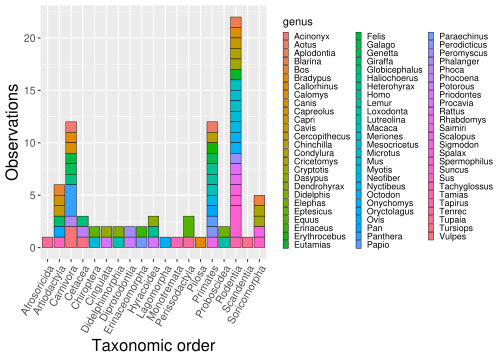
\includegraphics{5-ggplot2_kevin_files/figure-pdf/unnamed-chunk-23-1.pdf}

\begin{itemize}
\tightlist
\item
  Assign that last plot to an object called \texttt{obds\_msleep}.
\end{itemize}

\begin{Shaded}
\begin{Highlighting}[]
\NormalTok{obds\_msleep }\OtherTok{\textless{}{-}} \FunctionTok{ggplot}\NormalTok{(msleep, }\FunctionTok{aes}\NormalTok{(order)) }\SpecialCharTok{+}
  \FunctionTok{geom\_bar}\NormalTok{(}\FunctionTok{aes}\NormalTok{(}\AttributeTok{fill =}\NormalTok{ genus), }\AttributeTok{color =} \StringTok{"black"}\NormalTok{, }\AttributeTok{size =} \FloatTok{0.2}\NormalTok{) }\SpecialCharTok{+}
  \FunctionTok{labs}\NormalTok{(}\AttributeTok{x =} \StringTok{"Taxonomic order"}\NormalTok{, }\AttributeTok{y =} \StringTok{"Observations"}\NormalTok{) }\SpecialCharTok{+}
  \FunctionTok{theme}\NormalTok{(}
    \AttributeTok{axis.text.x =} \FunctionTok{element\_text}\NormalTok{(}\AttributeTok{size =} \FunctionTok{rel}\NormalTok{(}\FloatTok{1.2}\NormalTok{), }\AttributeTok{angle =} \DecValTok{60}\NormalTok{, }\AttributeTok{hjust =} \DecValTok{1}\NormalTok{, }\AttributeTok{vjust =} \DecValTok{1}\NormalTok{),}
    \AttributeTok{axis.text.y =} \FunctionTok{element\_text}\NormalTok{(}\AttributeTok{size =} \FunctionTok{rel}\NormalTok{(}\FloatTok{1.2}\NormalTok{)),}
    \AttributeTok{axis.title =} \FunctionTok{element\_text}\NormalTok{(}\AttributeTok{size =} \FunctionTok{rel}\NormalTok{(}\FloatTok{1.5}\NormalTok{)),}
    \AttributeTok{legend.key.size =} \FunctionTok{unit}\NormalTok{(}\DecValTok{2}\NormalTok{, }\StringTok{"mm"}\NormalTok{)}
\NormalTok{    ) }\SpecialCharTok{+}
  \FunctionTok{guides}\NormalTok{(}\AttributeTok{fill =} \FunctionTok{guide\_legend}\NormalTok{(}\AttributeTok{ncol =} \DecValTok{3}\NormalTok{))}
\end{Highlighting}
\end{Shaded}

\section{Exercise}\label{exercise-4}

\subsection{Plotting grid}\label{plotting-grid}

\begin{itemize}
\item
  Collate the plots that we assigend to objects through the day, as a
  single plot.

  \begin{itemize}
  \item
    Plots: \texttt{obds\_diamonds}, \texttt{obds\_chickweight},
    \texttt{obds\_msleep}.
  \item
    Methods: \texttt{cowplot::plot\_grid()}, \texttt{patchwork},
    \texttt{gridExtra::grid.arrange()}.
  \end{itemize}
\end{itemize}

Using \texttt{cowplot}.

\begin{Shaded}
\begin{Highlighting}[]
\NormalTok{first\_row }\OtherTok{\textless{}{-}}\NormalTok{ cowplot}\SpecialCharTok{::}\FunctionTok{plot\_grid}\NormalTok{(}
\NormalTok{  obds\_diamonds, obds\_chickweight,}
  \AttributeTok{ncol =} \DecValTok{2}
\NormalTok{)}
\end{Highlighting}
\end{Shaded}

\begin{verbatim}
`geom_smooth()` using method = 'gam' and formula = 'y ~ s(x, bs = "cs")'
\end{verbatim}

\begin{Shaded}
\begin{Highlighting}[]
\NormalTok{second\_row }\OtherTok{\textless{}{-}}\NormalTok{ cowplot}\SpecialCharTok{::}\FunctionTok{plot\_grid}\NormalTok{(}
\NormalTok{  obds\_msleep, }\AttributeTok{ncol =} \DecValTok{1}
\NormalTok{)}
\NormalTok{super\_plot }\OtherTok{\textless{}{-}}\NormalTok{ cowplot}\SpecialCharTok{::}\FunctionTok{plot\_grid}\NormalTok{(}
\NormalTok{  first\_row, second\_row,}
  \AttributeTok{nrow =} \DecValTok{2}
\NormalTok{)}
\NormalTok{super\_plot}
\end{Highlighting}
\end{Shaded}

\includegraphics{5-ggplot2_kevin_files/figure-pdf/unnamed-chunk-25-1.pdf}

Using \texttt{patchwork}.

\begin{Shaded}
\begin{Highlighting}[]
\FunctionTok{library}\NormalTok{(patchwork)}
\NormalTok{(obds\_diamonds }\SpecialCharTok{+}\NormalTok{ obds\_chickweight) }\SpecialCharTok{/}\NormalTok{ obds\_msleep}
\end{Highlighting}
\end{Shaded}

\begin{verbatim}
`geom_smooth()` using method = 'gam' and formula = 'y ~ s(x, bs = "cs")'
\end{verbatim}

\includegraphics{5-ggplot2_kevin_files/figure-pdf/unnamed-chunk-26-1.pdf}

Using \texttt{gridExtra}.

\begin{Shaded}
\begin{Highlighting}[]
\FunctionTok{library}\NormalTok{(gridExtra)}
\FunctionTok{grid.arrange}\NormalTok{(}
  \AttributeTok{grobs=}\FunctionTok{list}\NormalTok{(obds\_diamonds, obds\_chickweight, obds\_msleep),}
  \AttributeTok{layout\_matrix =} \FunctionTok{rbind}\NormalTok{(}\FunctionTok{c}\NormalTok{(}\DecValTok{1}\NormalTok{, }\DecValTok{2}\NormalTok{),}
                        \FunctionTok{c}\NormalTok{(}\DecValTok{3}\NormalTok{, }\DecValTok{3}\NormalTok{))}
\NormalTok{)}
\end{Highlighting}
\end{Shaded}

\begin{verbatim}
`geom_smooth()` using method = 'gam' and formula = 'y ~ s(x, bs = "cs")'
\end{verbatim}

\includegraphics{5-ggplot2_kevin_files/figure-pdf/unnamed-chunk-27-1.pdf}

\begin{itemize}
\tightlist
\item
  Export the new plot in a PDF file, and open it in a PDF viewer
  (e.g.~Adobe Acrobat Reader DC).
\end{itemize}

You will likely need a few attempts to fine-tune the width and height of
the output file.

\begin{Shaded}
\begin{Highlighting}[]
\FunctionTok{ggsave}\NormalTok{(}\StringTok{"final\_plot.pdf"}\NormalTok{, super\_plot, }\AttributeTok{width =} \DecValTok{12}\NormalTok{, }\AttributeTok{height =} \DecValTok{12}\NormalTok{)}
\end{Highlighting}
\end{Shaded}

\section{Exercise}\label{exercise-5}

\subsection{Pair programming}\label{pair-programming}

\begin{itemize}
\tightlist
\item
  Explore the data set \texttt{ggplot2::mpg} and generate the most
  informative plot that you can!
\end{itemize}

\begin{Shaded}
\begin{Highlighting}[]
\FunctionTok{ggplot}\NormalTok{(mpg, }\FunctionTok{aes}\NormalTok{(cty, hwy, }\AttributeTok{color =}\NormalTok{ year)) }\SpecialCharTok{+}
  \FunctionTok{geom\_abline}\NormalTok{(}\AttributeTok{slope =} \DecValTok{1}\NormalTok{, }\AttributeTok{intercept =} \DecValTok{0}\NormalTok{) }\SpecialCharTok{+}
  \FunctionTok{geom\_point}\NormalTok{(}\AttributeTok{size =} \FloatTok{0.5}\NormalTok{) }\SpecialCharTok{+}
  \FunctionTok{facet\_wrap}\NormalTok{(}\SpecialCharTok{\textasciitilde{}}\NormalTok{manufacturer)}
\end{Highlighting}
\end{Shaded}

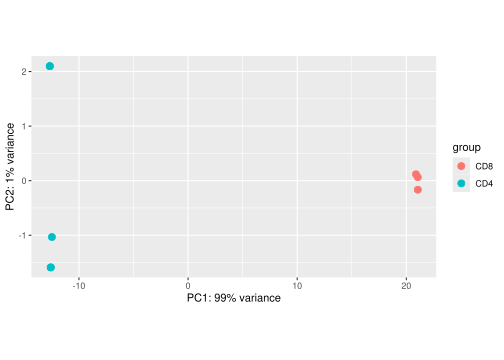
\includegraphics{5-ggplot2_kevin_files/figure-pdf/unnamed-chunk-29-1.pdf}




\end{document}
